\documentclass[../main.tex]{subfiles}
\graphicspath{{\subfix{../images/}}}
\usepackage{subfiles}
\usepackage{subfig}

\begin{document}
    \subsection{Moving Averages and Autoregressive Models}
        In this section, we delve further into the modeling of stochastic processes, particularly through Moving Averages (MA), Autoregressive (AR) models, and their combinations. To make an informed choice among these options, it is crucial to comprehend the correlogram of our variable. Hence, we will now explore the concept of correlograms.\par

        Initially, let's consider a scenario where our time series observations, denoted as $x_1$, $x_2$, ..., $x_N$, are independent and identically distributed random variables. In this case, it can be demonstrated that the expected value for the estimator $r_k$ (representing the autocorrelation coefficient $\rho(k)$) is approximately $-\frac{1}{N}$, while the variance of $r_k$ is approximately $\frac{1}{N}$.\par
        
        This statistical insight allows us to assess the randomness of a time series by employing the 95\% confidence interval of the correlogram coefficients, which can be calculated as $\pm \frac{1.96}{\sqrt{N}}$. Consequently, coefficients falling within this interval suggest a purely random process, while those outside the interval are deemed significant. However, it is important to note that depending on the size of $N$, approximately 5\% of the coefficients may fall outside the interval even in a random process.\par
        
        By understanding and analyzing the correlogram coefficients, we gain valuable insights into the presence of autocorrelation and the degree of randomness exhibited by the time series. This knowledge aids in selecting appropriate modeling approaches and making meaningful interpretations of the data.\par

        In addition, the correlogram of a time series provides valuable insights into its stationarity and underlying process. When the correlogram coefficients do not decay quickly, it indicates that the series is non-stationary and requires differencing to achieve stationarity. On the other hand, if the correlogram exhibits a sudden cut-off at a specific lag, it suggests a MA(q) process. In contrast, an AR process is characterized by a combination of sinusoids and a damped exponential pattern in the correlogram. Mixed Autoregressive Moving Averages (ARMA) models follow a similar pattern as AR models, having a tendency to display a damped decay and sinusoidal behavior instead of a distinct cut-off. By analyzing the correlogram, we can identify the nature of the underlying process and select an appropriate modeling approach accordingly.\par

        When using a AR(p) model, the fitting of the data can be done as a simple regression model to find the coefficients \{$\hat{\alpha}_1$, ..., $\hat{\alpha}_p$\} that best fit equation \ref{eq:lin_reg}. To determine the order of such process, looking at the ac.f. might not be so insightful as in the MA case. Because of that, we can use what is called the \textbf{partial autocorrelation function}, that measures the excess correlation at lag $p$ that is not accounted for in lag $p-1$. In the partial autocorrelation function, the properties of the MA and AR are inverted when compared to the normal ac.f., meaning that now the AR process will have a cut-off at lag p, while the MA one will tend to attenuate slowly.
        
        \begin{equation}
            \label{eq:lin_reg}
            (X_t-\bar{x}) = \hat{\alpha}_1(X_{t-1}-\bar{x}) + ... + \hat{\alpha}_p(X_{t-p}-\bar{x})
        \end{equation}

        Fitting a MA process is a little harder because efficient explicit estimators cannot be found. Assuming a process of the from

        \begin{equation}
            \label{eq:ma}
            X_t = \mu + Z_t + \beta_1Z_{t-1} + ... + + \beta_qZ_{t-q}
        \end{equation}

        we would start with an initial guess for the values of $\mu$, $\beta_1$, ..., $\beta_q$ and then iteratively improve upon it by means of optimization procedures that minimize the residual sum of squares. Feating ARMA and ARIMA models follow similar paths, typically involving iteratively optimizing the residue. Because of this added complexity for fitting MA models when compared to AR, many times AR ones are prefered, even at the expense of more parameters.\par

        Applying this concepts to our study case, we can see in figure \ref{fig:acf} the autocorrelation and partial autocorrelation functions for our Heart Rate data. As we can see, the autocorrelation shows a very slow decay, meaning that the series is most likely not stationary and should be differentiated. Doing that, we get the plots on the right, that show a different picture. With that, we can see that mostly only one lag is relevant both for the AR and the MA (the other values that lie outside the 95\% confidence interval in farther lags are probably only due to chance, as was mentioned before that approximately 5\% of the coefficients would lie outside the bounds even in completely random series). With these informations, we know that a ARIMA model should be considered (as the data is not stationary) taking into account only a single lag. \par 

        \begin{figure}[h]
            \begin{center}
            \centering
            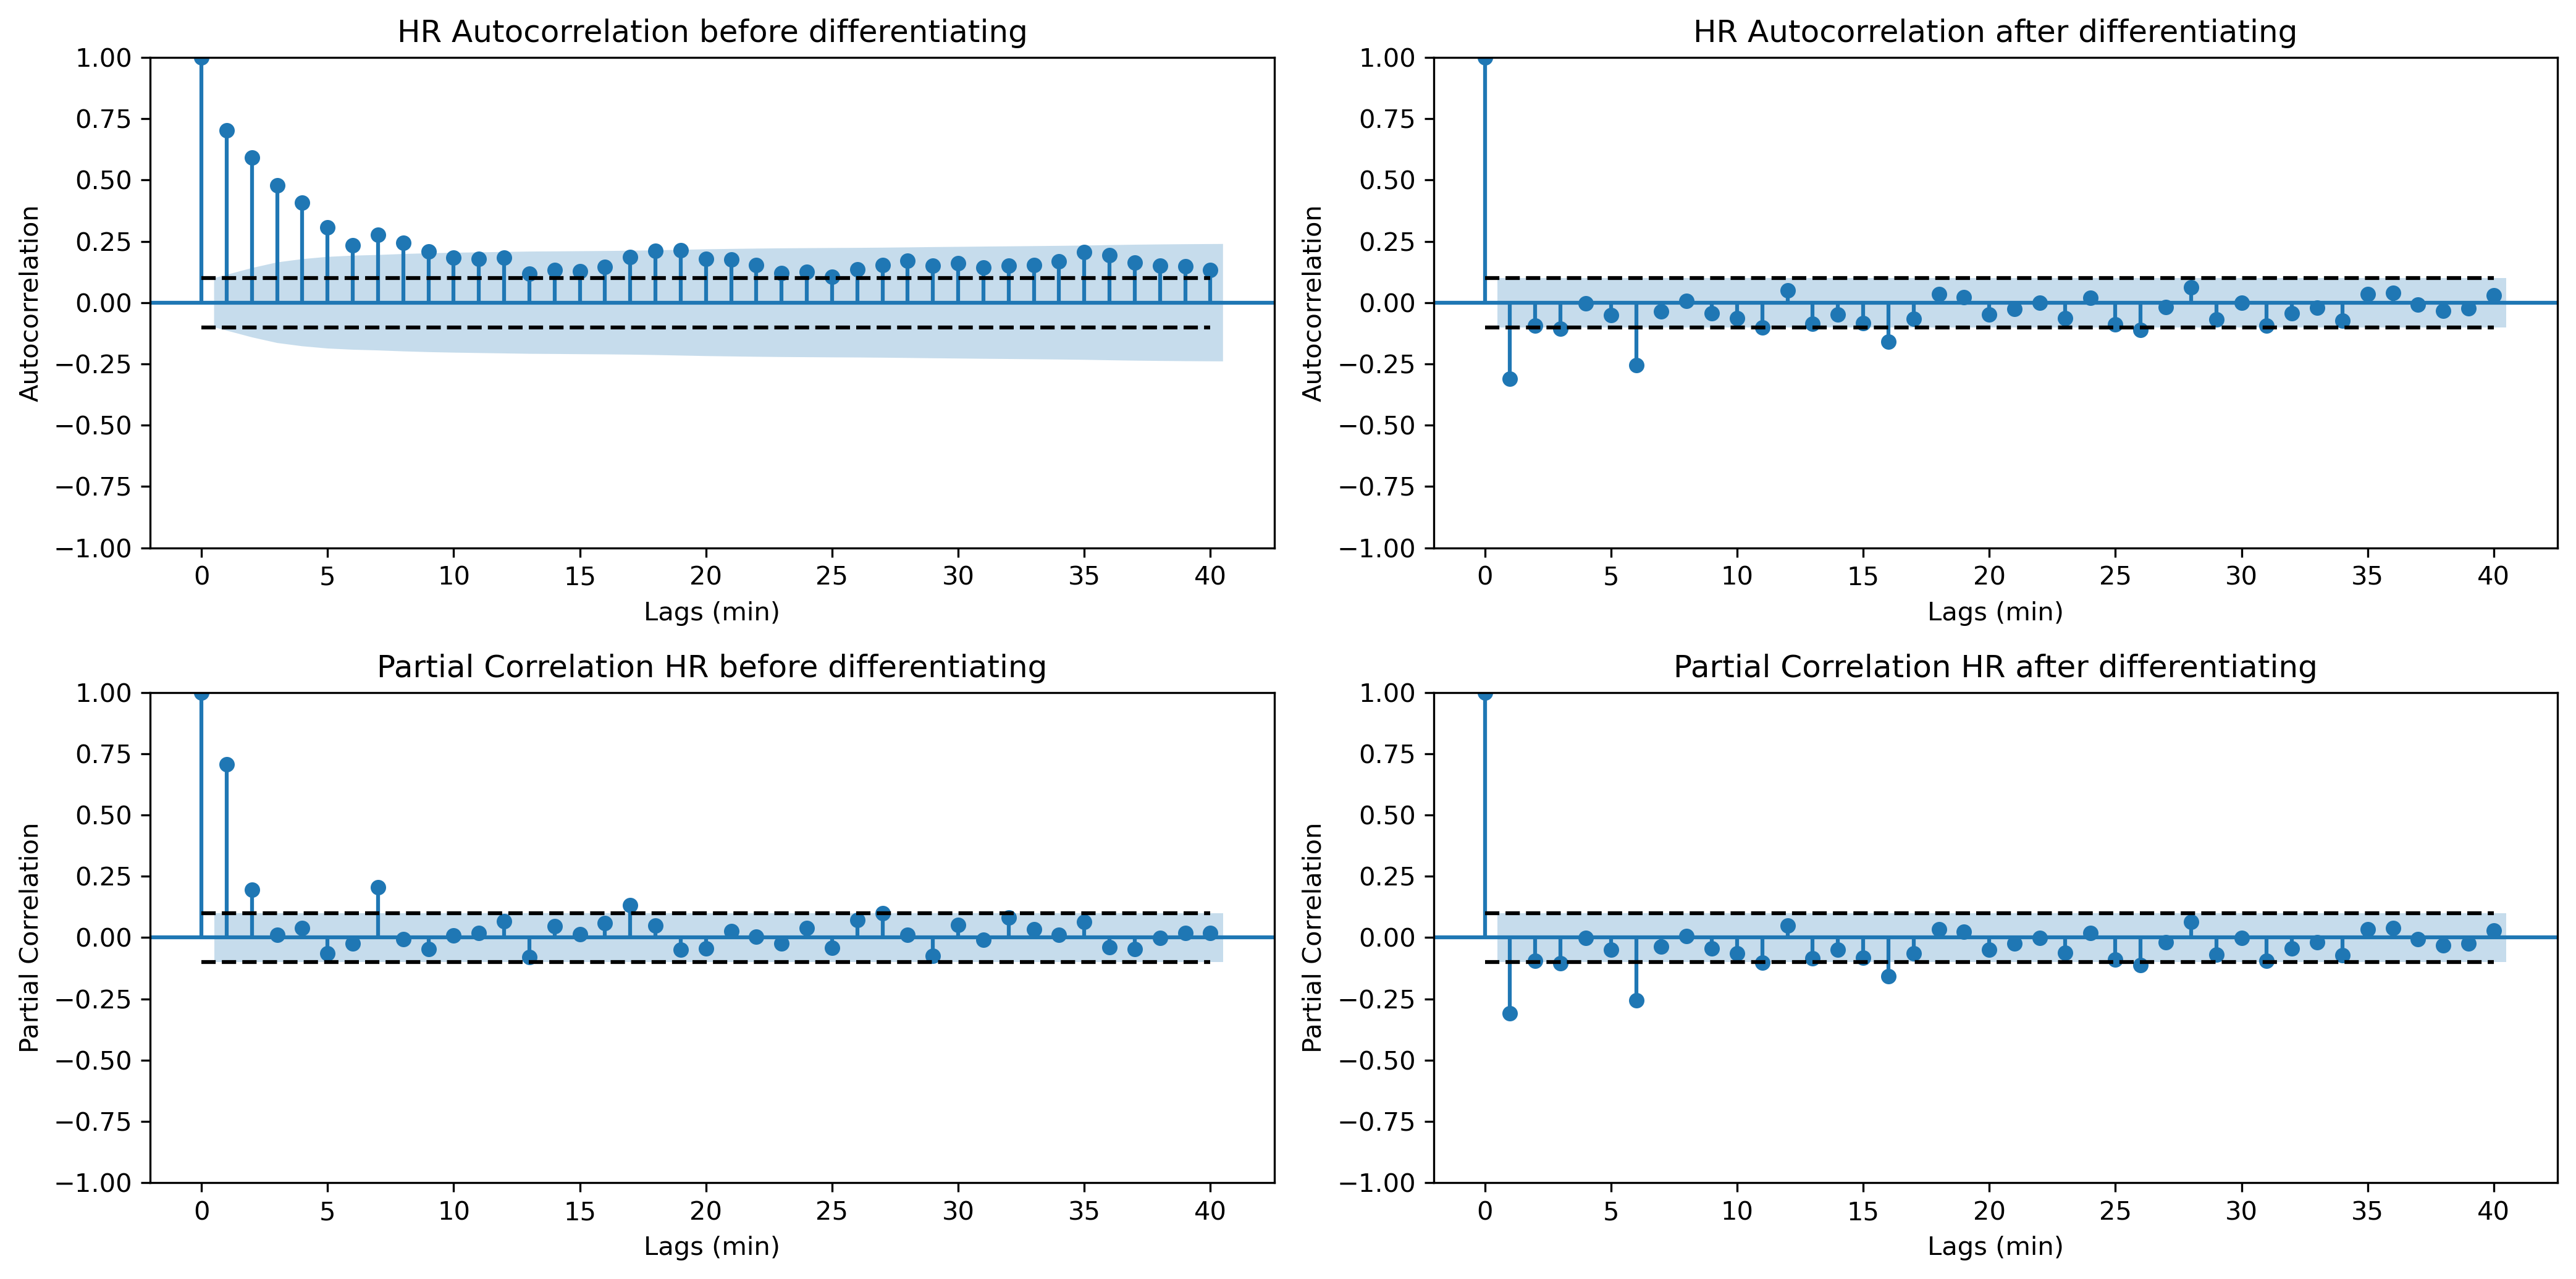
\includegraphics[width={\columnwidth}]{images/acf.png}
            \caption{Plot of the autocorrelation and partial autocorrelation for the raw and differentiated HR time series data. The dashed lines mark the 95\% confidence interval for the coefficients.}
            \label{fig:acf}
            \end{center}
        \end{figure}

        With this information, we can fit an ARIMA model using 1 lag for the MA and one lag for the AR. We can see from Figure \ref{fig:arima} that the model tends to fit pretty well to the data, although it tended not to follow the data on the peaks. Considering the non normalized data, it achieved an MSE of $71.3$.
        
        \begin{figure}[h]
            \begin{center}
            \centering
            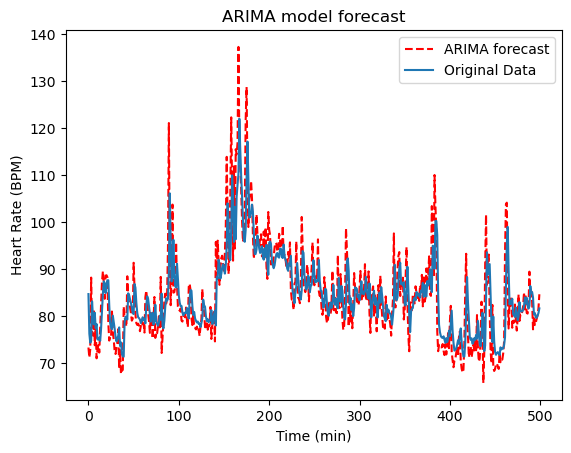
\includegraphics[width={\columnwidth}]{images/ARIMA.png}
            \caption{ARIMA model forecast compared to original time series data for the HR of the Lawson dataset using a period not used during the parameter estimation.}
            \label{fig:arima}
            \end{center}
        \end{figure}

        From the ac.f. and pac.f. of the residuals of the ARIMA model (the difference between the original series and the predicted one) shown in Figure \ref{fig:res_arima}, it is possible to see that no correlation appears to be left, meaning the model fitted was with the right specifications (remember that even for a completely random series some coefficients are expected to be above the threshold by pure chance).

        \begin{figure}[h]
            \begin{center}
            \centering
            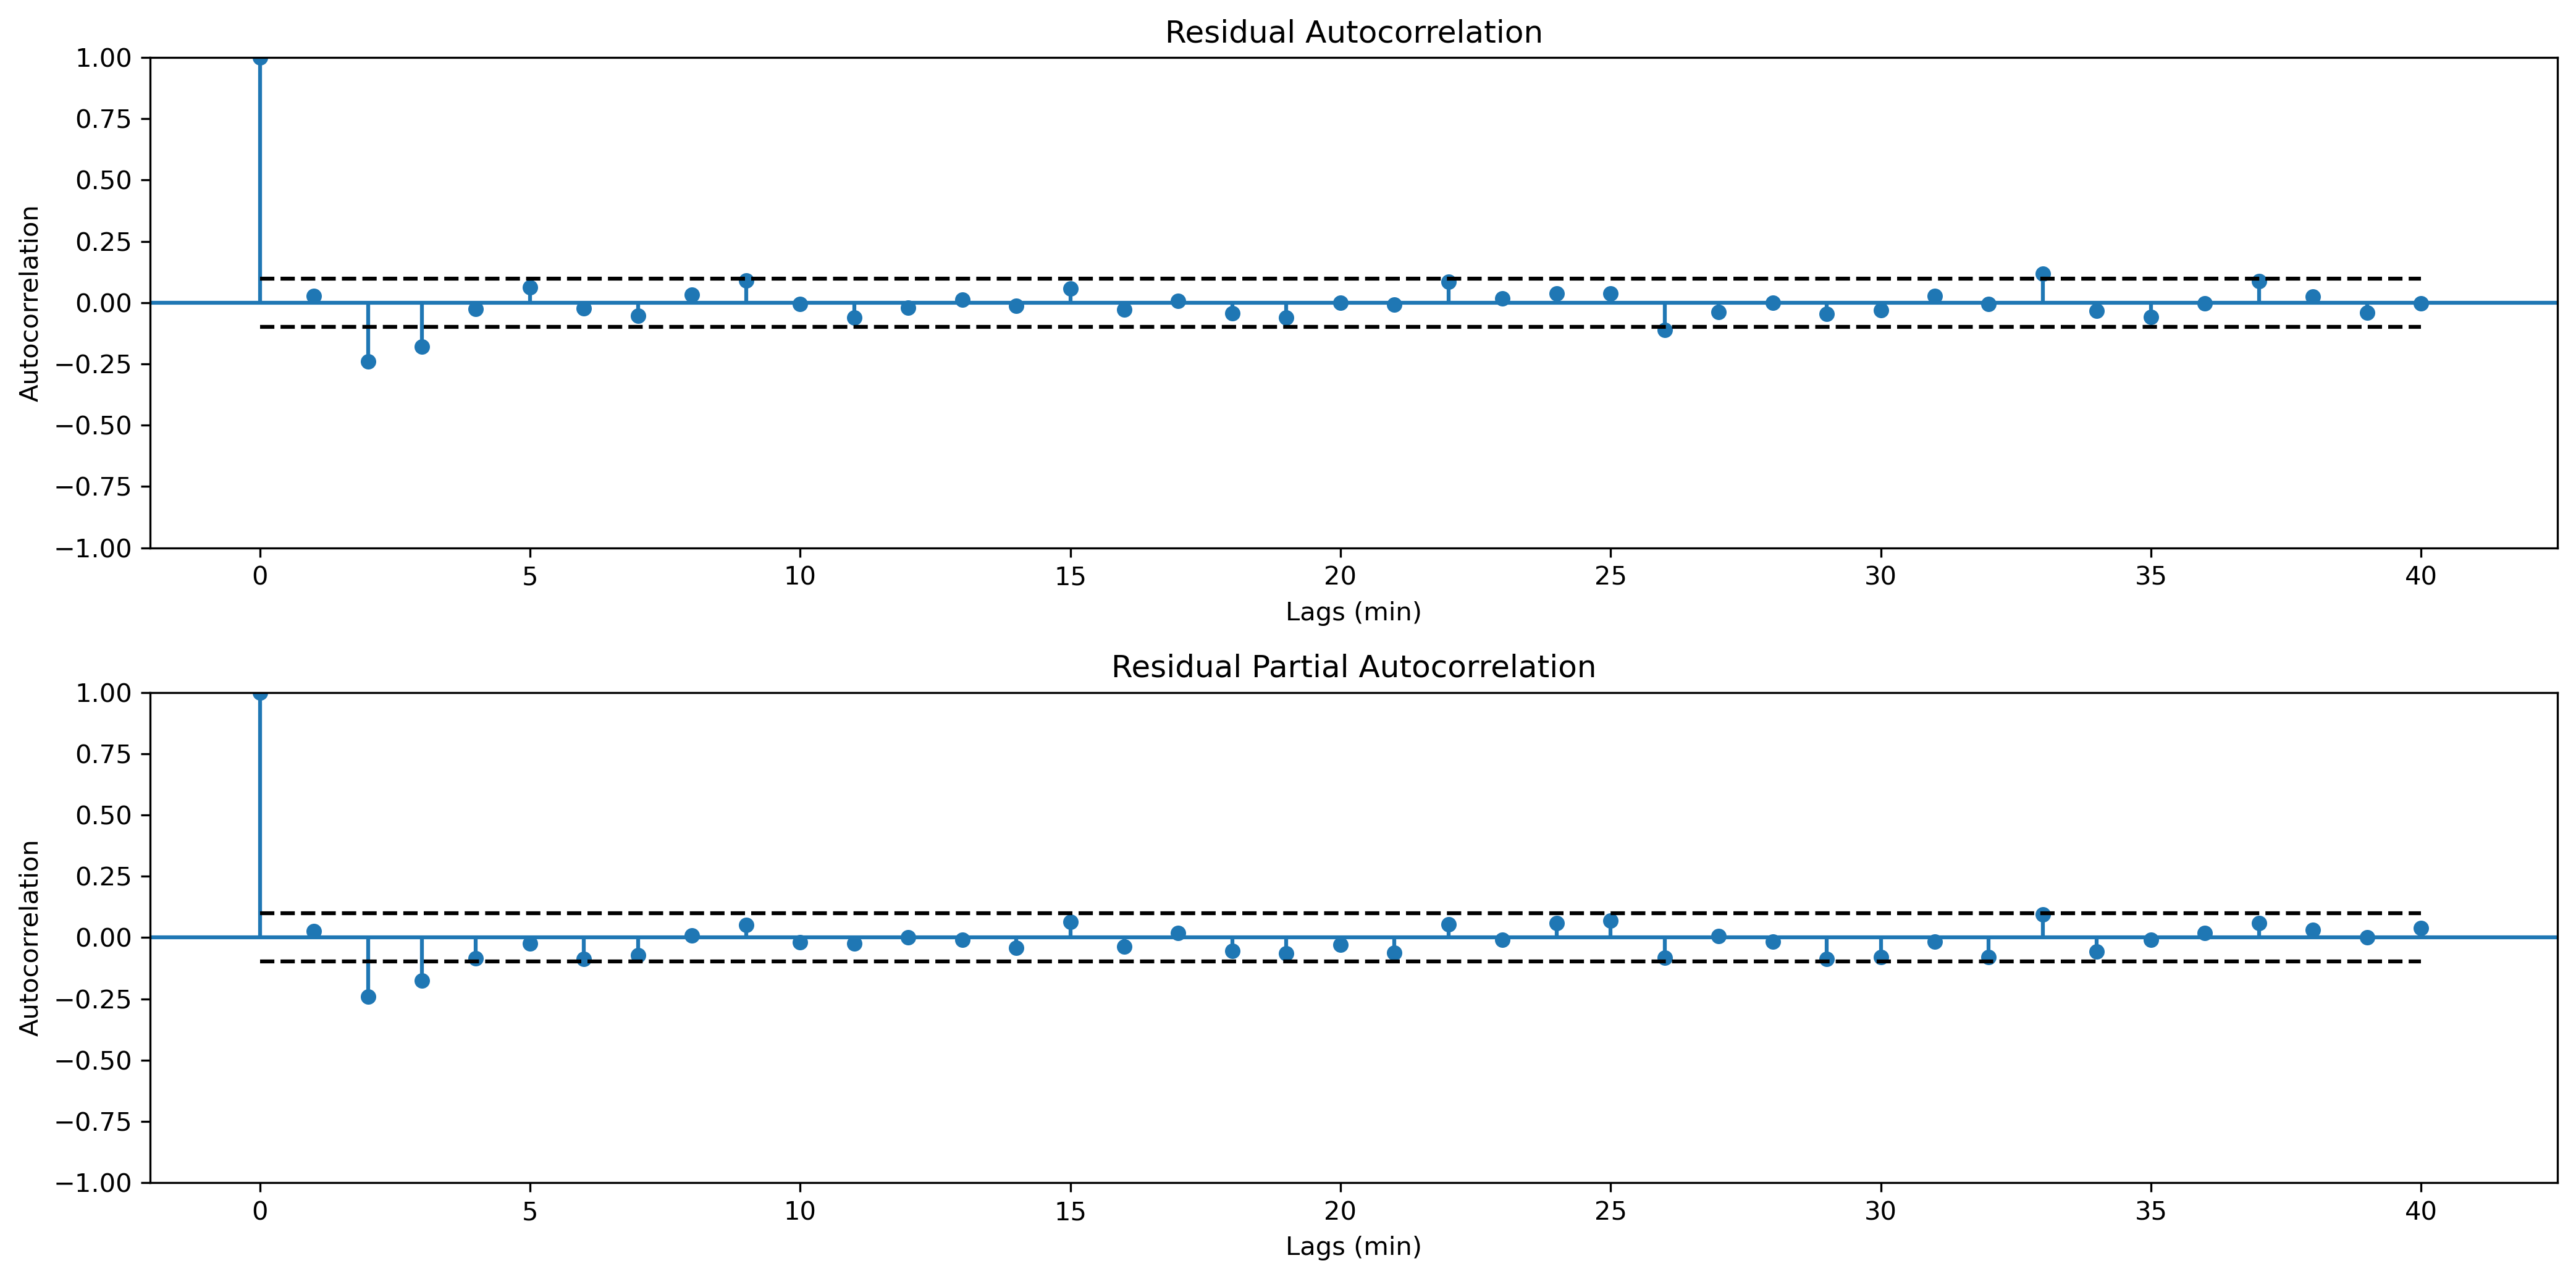
\includegraphics[width={\columnwidth}]{images/res_ARIMA.png}
            \caption{Autocorrelation and Partial Autocorrelation for the residuals from the ARIMA model.}
            \label{fig:res_arima}
            \end{center}
        \end{figure}

    \subsection{Multivariate Forecasting}
        For now, we have only been considering infering the future values of the series based on the previous measured ones, but what if we have access to other features as well? Take for instance the case of the Lawson data, where there are measurements of activity and temperature, as well as the heart rate. By looking more into the data, we can see for example that the activity is strongly correlated to the heart rate, specially when considering their averages over a time period. Figure \ref{fig:corr} shows this relation between the variables. Another relation that can be observed from the data is regarding the temperature, where higher temperatures tend, on average, to result in lower heart rates. This can be seen in Figure \ref{fig:temp}. By considering this external variables to the series that are still clearly related to the future values of it, it is reasonable to assume that by including them in our forecasting model, the results would be better. \par

        \begin{figure}[h]
            \begin{center}
            \centering
            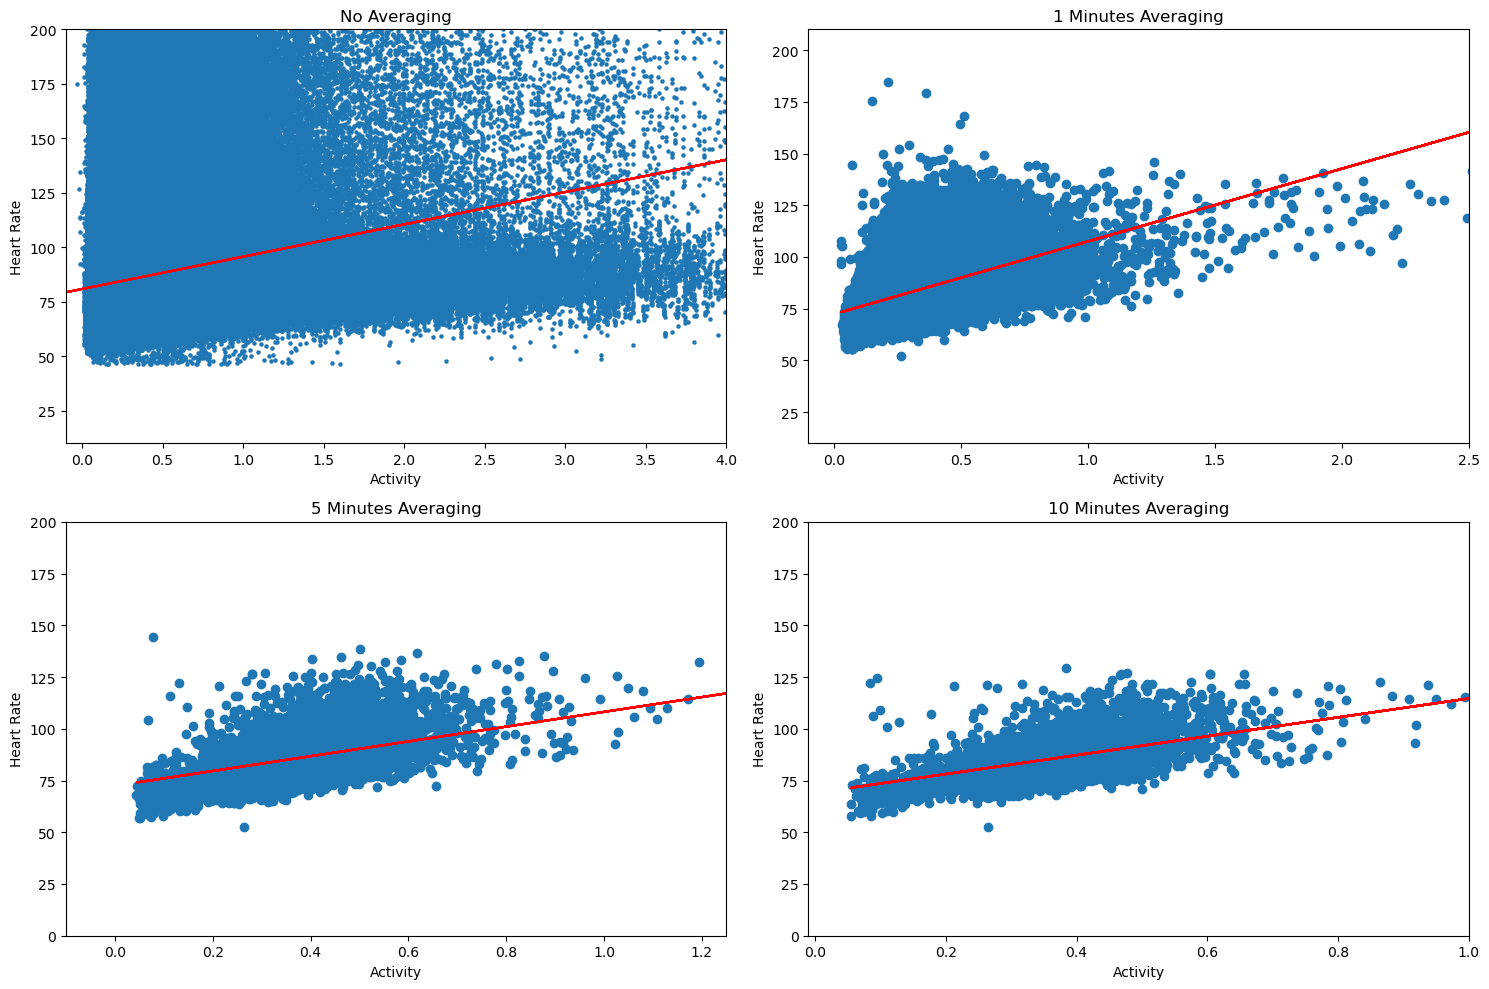
\includegraphics[width={\columnwidth}]{images/activity_hr_correlation.png}
            \caption{Plot of the heart rate as a function of the activity value for different averaging times. It is clear that both variables are highly correlated, and that the higher the averaging window the more linearly correlated this relationship becomes.}
            \label{fig:corr}
            \end{center}
        \end{figure}

        \begin{figure}[h]
            \begin{center}
            \centering
            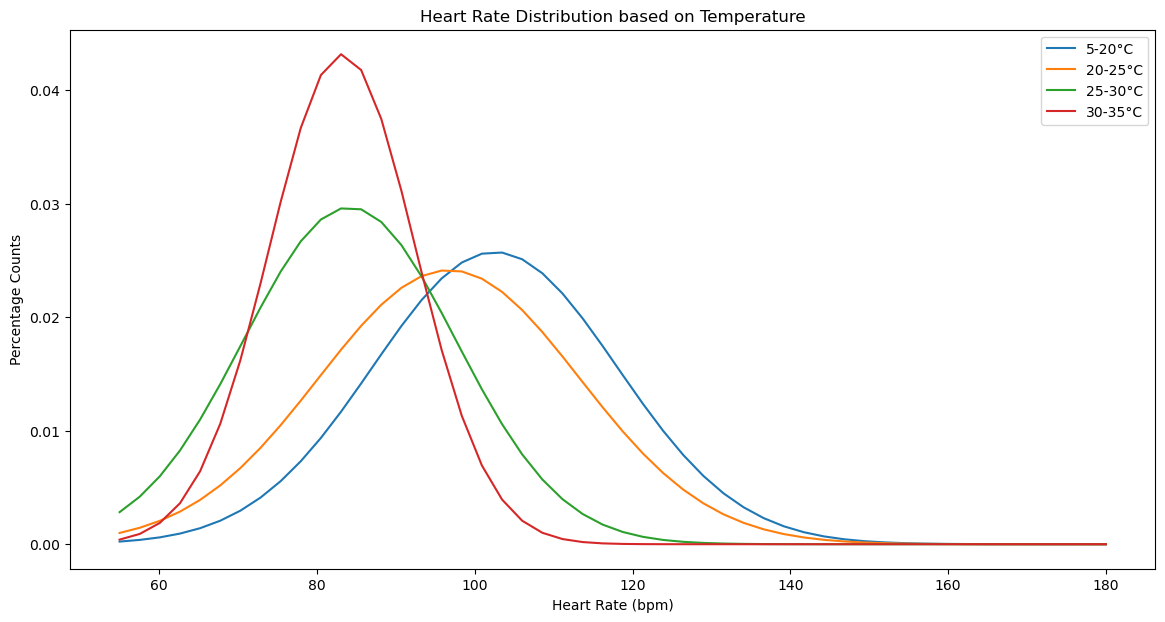
\includegraphics[width={\columnwidth}]{images/temperature.png}
            \caption{Histogram showing the relationship between the heart rate and different temperature ranges. As can be seen, the higher the temperature, the lower is the heart rate on average. We can see also that the ranges 25-30$^\circ C$ and 30-35$^\circ C$ have similar averages, but the 25-30$^\circ C$ is much more spreadout.}
            \label{fig:temp}
            \end{center}
        \end{figure}

        
\end{document}